\clearpage % Rozdziały zaczynamy od nowej strony.
\section{Realizacja Pracowni}

\subsection{Harmonogram prac}

Na początku semestru sporządzono harmonogram prac, który został przedstawiony w tabeli \ref{table:harmonogram}.

\begin{longtable}{| m{0.67\linewidth} | r |}
    \caption{Harmonogram prac.}
    \label{table:harmonogram} \\

    \hline
    % Nagłówek tabeli wyrównujemy do środka
    \multicolumn{1}{|c|}{Kamień milowy} & \multicolumn{1}{c|}{Przewidywana data ukończenia} \\ \hline\hline \endfirsthead \endfoot
    \hline \endlastfoot

    Zamodelowanie zdarzeń biznesowych przy pomocy techniki Event Storming & 27.03.2023 \\ \hline
    Wstępny wybór technologii & 17.04.2023 \\ \hline
    Przygotowanie środowiska programistycznego & 24.04.2023 \\ \hline
    Weryfikacja wykorzystania wybranych technologii & 8.05.2023 \\ \hline
    Ustalenie wymagań funkcjonalnych i niefunkcjonalnych & 22.05.2023 \\ \hline
    Wykonanie makiet interfejsu użytkownika & 5.06.2023 \\ \hline
    Ustalenie formatów i technik wymiany danych & 12.06.2023 \\ \hline
    Przygotowanie mechanizmów uwierzytelniania i autoryzacji użytkowników & 19.06.2023 \\ \hline
    Zaprojektowanie architektury i infrastruktury aplikacji & 26.06.2023 \\ \hline
    Główna implementacja & 2.10.2023 \\ \hline
    Wdrożenie produkcyjne aplikacji & 9.10.2023 \\ \hline
    Przygotowanie i wykonanie automatycznych testów akceptacyjnych & 23.10.2023 \\ \hline
    Przygotowanie i wykonanie automatycznych testów wydajnościowych & 6.11.2023\\ \hline
    Przygotowanie raportu z wydajności i skalowalności systemu & 13.11.2023 \\ \hline
    Przygotowanie wstępnego tekstu pracy inżynierskiej & 18.12.2023 \\ \hline
    Przygotowanie finalnego tekstu pracy inżynierskiej & 8.01.2024 \\ \hline
    Złożenie pracy inżynierskiej & 15.01.2024 \\ \hline
\end{longtable}

Zakres Pracowni Dyplomowej 1 zakończył się wraz z ukończeniem kamienia milowego \textit{Wykonanie makiet interfejsu użytkownika}.

% Podrozdział pierwszego poziomu
\subsection{Zamodelowanie zdarzeń biznesowych}

\subsubsection{Event Storming}

W celu zrozumienia procesów oraz zidentyfikowania potencjalnych mikroserwisów w tworzonej aplikacji przeprowadzono sesję Event Stormingu \cite{eventstorming}. Metoda ta umożliwia wizualizację i modelowanie procesów biznesowych w ramach systemu, co jest kluczowe przy tworzeniu złożonych systemów informatycznych. W niniejszym rozdziale przedstawione zostaną wyniki sesji Event Stormingu, która została przeprowadzona z wykorzystaniem narzędzia Miro.

\subsubsection{Narzędzie Miro}

Miro \cite{miro} to interaktywna platforma webowa, umożliwiająca tworzenie tablic z notatkami, rysunkami i diagramami. Wybór tego narzędzia był podyktowany jego prostotą użytkowania oraz możliwościami wizualizacji efektów.

\subsubsection{Identyfikacja kontekstów granicznych (Bounded Context)}

W wyniku sesji Event Stormingu zidentyfikowano pięć kontekstów granicznych (Bounded Context \cite{boundedcontext}), które będą kluczowe dla tworzonej aplikacji. Są to:

\textbf{Restaurant} (\textit{Restauracja}) - obejmuje zarządzanie restauracjami, menu oraz definicją i dostępnością produktów,

\textbf{Order} (\textit{Zamówienie}) - odpowiada za proces zamówienia, jego składanie, modyfikowanie, anulowanie oraz koordynuje cały proces przygotowania zamówienia do momentu dostawy,

\textbf{Delivery} (\textit{Dostawa}) - koncentruje się na logistyce dostaw, monitorowaniu statusu dostawy oraz komunikacji z dostawcą. Zarządza również bazą dostawców,

\textbf{Payment} (\textit{Płatność}) - zarządza procesem płatności, obejmuje różne metody płatności oraz obsługę transakcji. Obsługuje wszelkie rozliczenia w ramach systemu,

\textbf{Invoice} (\textit{Faktura}) - odpowiada za generowanie faktur i rachunków dla użytkowników, restauracji oraz dostawców.

\subsubsection{Analiza procesów}

Każdy z wyżej wymienionych kontekstów granicznych został poddany analizie procesów, które występują w ramach danej domeny. W trakcie analizy zidentyfikowano następujące kluczowe procesy:

\begin{itemize}
    \item Restaurant
    \begin{itemize}
        \item Dodanie nowej restauracji
        \item Aktualizacja informacji o restauracji, np. godziny otwarcia lub opis
        \item Dodanie/aktualizacja menu oraz cennika
        \item Zmiana dostępności restauracji (otwarcie/zamknięcie)
        \item Przyjęcie lub odrzucenie zamówienia przez restaurację
        \item Oznaczenie zamówienia jako gotowe do odbioru
    \end{itemize}
    
    \item Order
    \begin{itemize}
        \item Utworzenie nowego zamówienia
        \item Modyfikacja zamówienia (dodanie/usunięcie produktu)
        \item Anulowanie zamówienia
        \item Finalizacja zamówienia
    \end{itemize}
    
    \item Delivery
    \begin{itemize}
        \item Dodanie nowego dostawcy
        \item Aktualizacja informacji o dostawcy
        \item Zmiana dostępności dostawcy
        \item Przypisanie dostawcy do zamówienia
        \item Wytyczenie trasy dostawy
        \item Odbiór zamówienia przez dostawcę
        \item Dostarczenie zamówienia do klienta
    \end{itemize}
    
    \item Payment
    \begin{itemize}
        \item Przyjęcie płatności za zamówienie
        \item Obsługa nieudanej płatności
        \item Rozliczenie płatności z dostawcą
        \item Rozliczenie płatności z restauracją
        \item Obsługa zwrotu płatności w przypadku anulowania zamówienia
        \item Wypłata środków do restauracji
        \item Wypłata środków do dostawcy
    \end{itemize}
    
    \item Invoice
    \begin{itemize}
        \item Generowanie faktury dla restauracji
        \item Generowanie faktury dla dostawcy
        \item Generowanie faktury dla zamawiającego
    \end{itemize}
\end{itemize}


\subsubsection{Reprezentacja graficzna}

Na rysunku \ref{fig:event-storming} przedstawiono fragment wyniku sesji Event Stormingu w postaci diagramu wygenerowanego przy pomocy narzędzia Miro.

\begin{figure}[!h]
    \centering 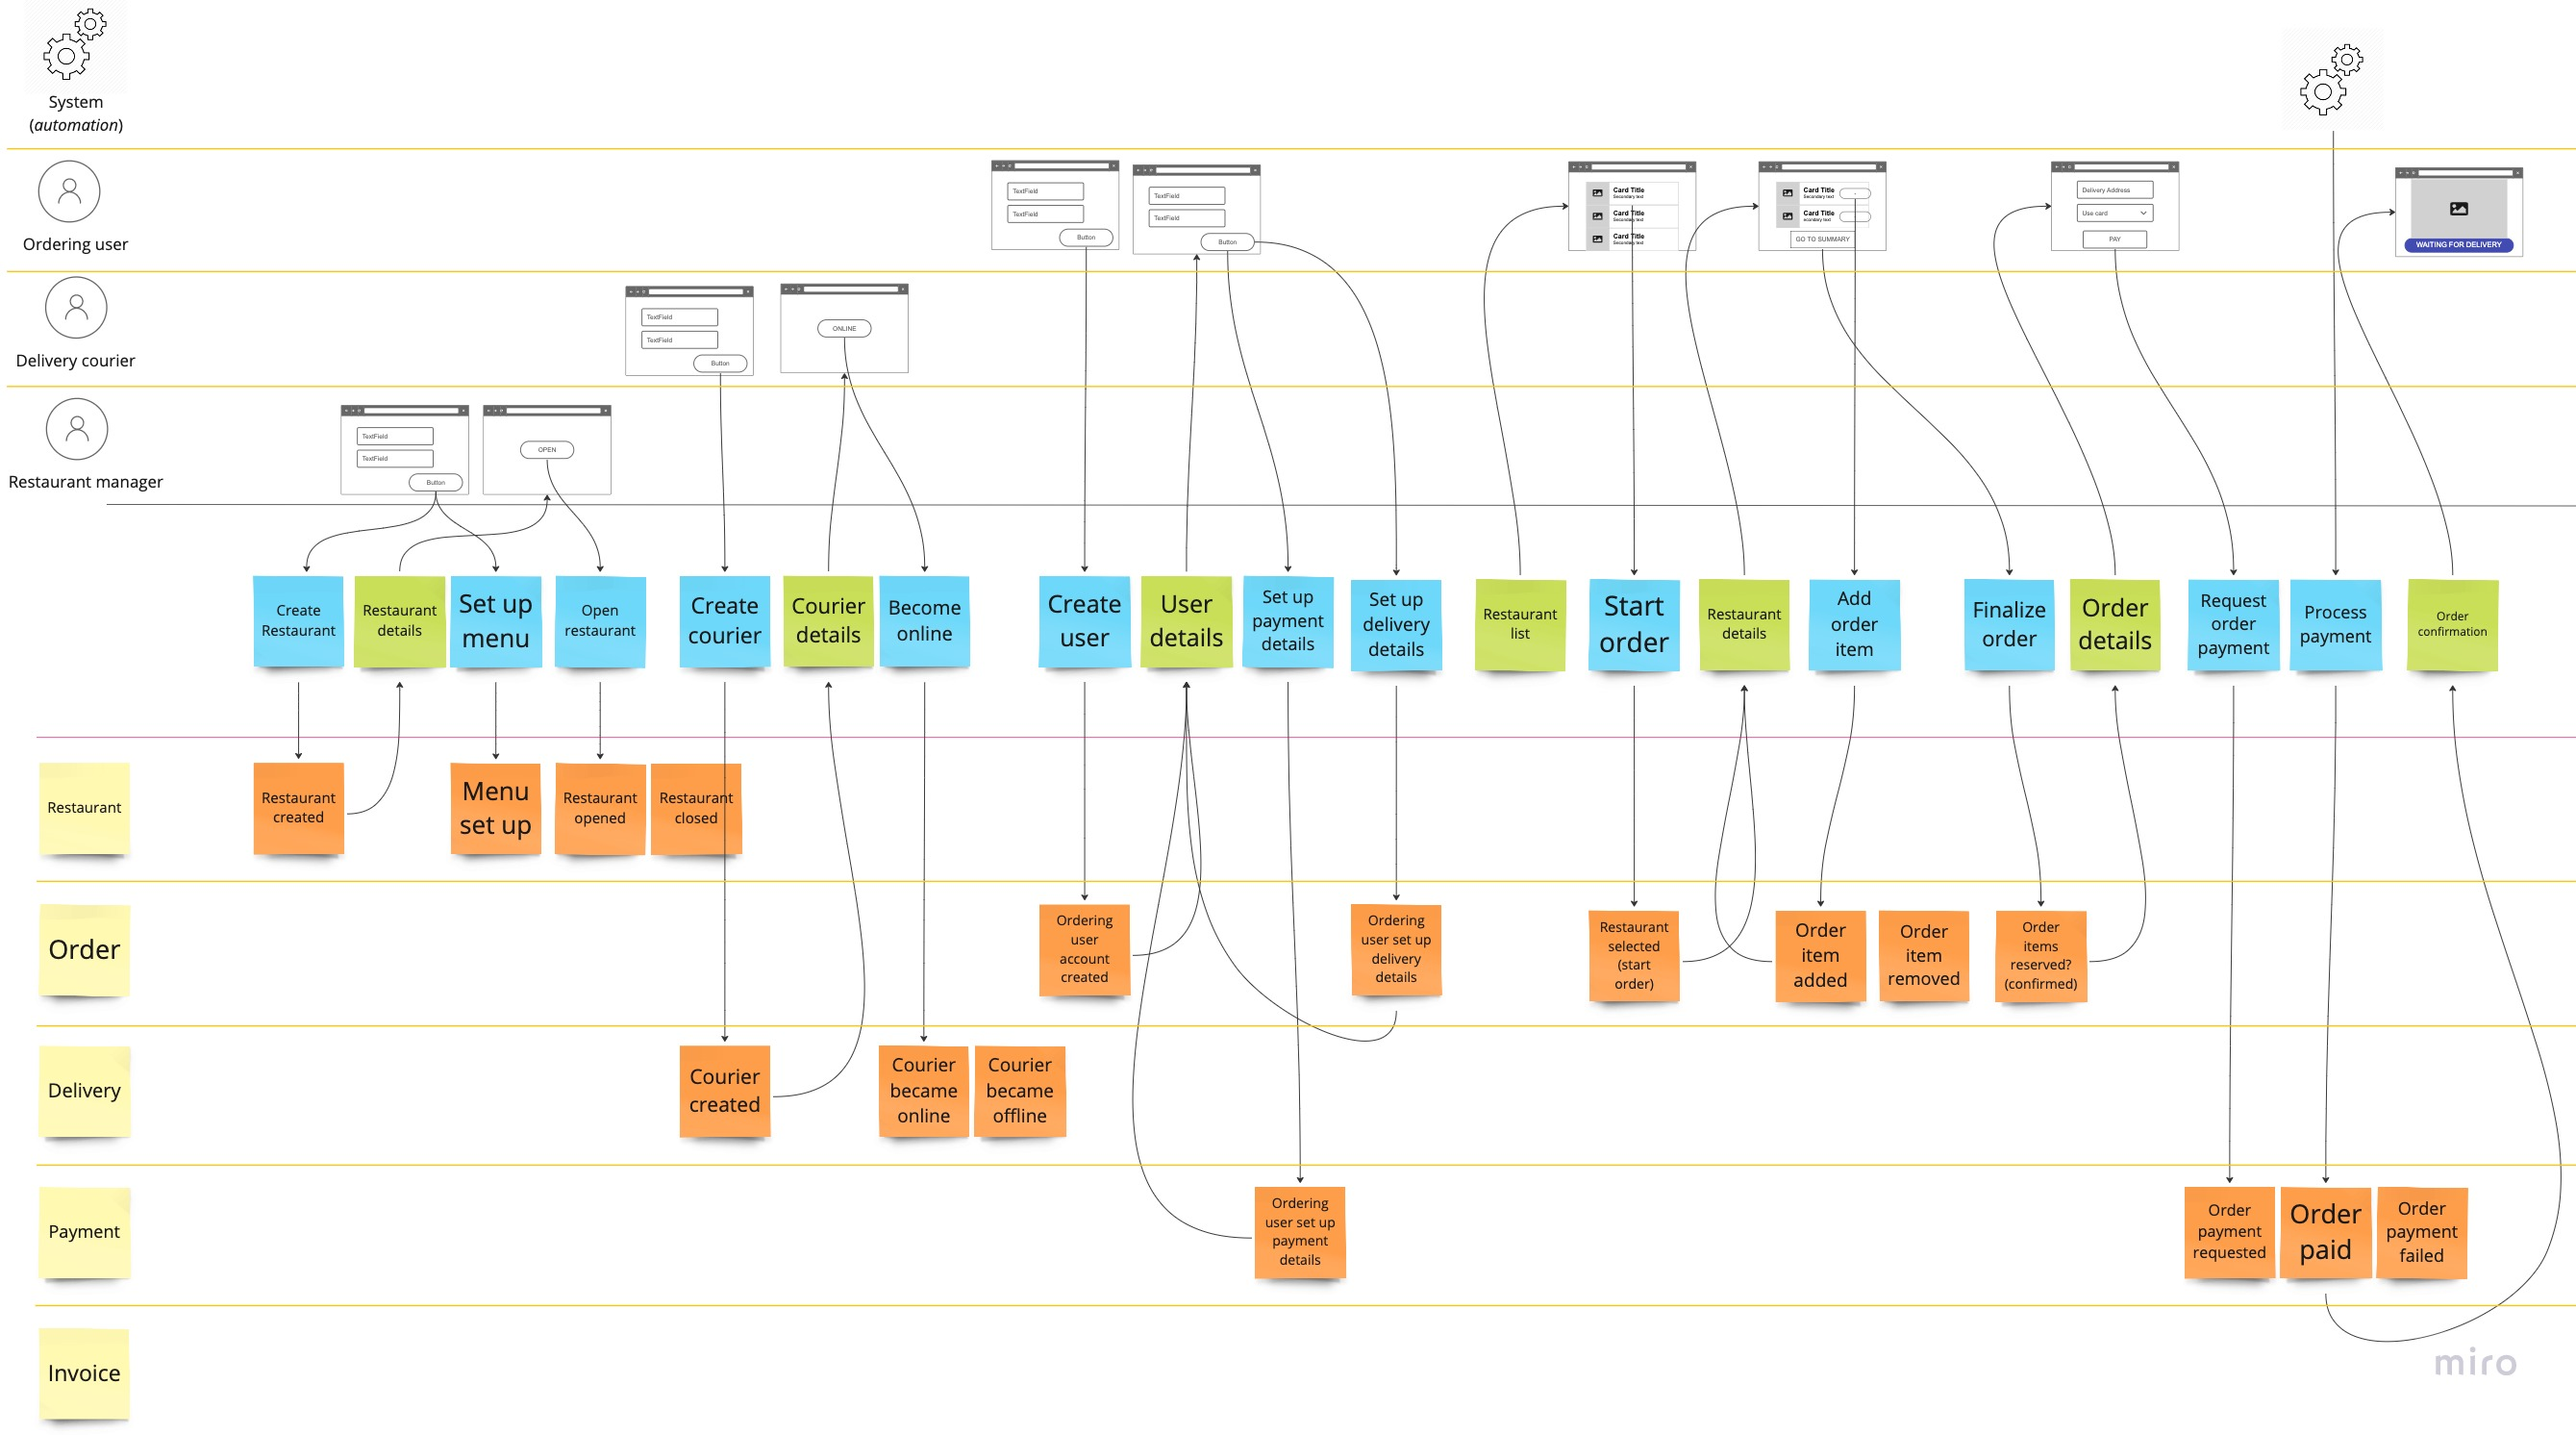
\includegraphics[width=1.0\linewidth]{event_storming_fragment.jpg}
    \caption{Reprezentacja graficzna efektów sesji Event Stormingu}
    \label{fig:event-storming}
\end{figure}



% Nagłówki kolejnych poziomów, dla zapełnienia spisu treści
\subsection{Wstępny wybór technologii}

Wstępny wybór technologii został dokonany na podstawie analizy wymagań funkcjonalnych i niefunkcjonalnych oraz doświadczenia Autora. 

W celu zapewnienia wydajności i skalowalności systemu zdecydowano się na architekturę opartą o zdarzenia. W tym celu wybrano framework Axon Framework \cite{axonframework}, który służy do tworzenia aplikacji opartych o techniki CQRS \cite{cqrs} i Event Sourcing \cite{eventsourcing}, które pomagają w procesie implementacji skalowalnych i łatwo utrzymywalnych złożonych systemów informatycznych. Dodatkowo Axon Framework jest zintegrowany z frameworkiem Spring Boot \cite{springboot}, który jest jednym z najpopularniejszych frameworków do tworzenia aplikacji na platformę JVM \cite{jvm}.

Jako, że baza danych przy zastosowaniu Event Sourcingu pełni jedynie funkcję magazynu danych w warstwie prezentacji, zastosowano dokumentową bazę NoSQL \cite{nosql} - MongoDB \cite{mongodb}. Wybór ten podyktowany jest głównie wydajnością i skalowalnością bazy danych oraz najbliższym rzeczywistości formacie danych - JSON \cite{json}. Identyczny format zastosowano w warstwie komunikacji pomiędzy komponentami.

W części klienckiej zastosowano bibliotekę do tworzenia webowych interfejsów graficznych - React \cite{react} wraz z pomocniczym frameworkiem Remix \cite{remix}, umożliwiającym przygotowywanie widoków po stronie serwera, co znacząco wpływa na wydajność rozwiązania.

\subsubsection{Część serwerowa}

Język programowania: Kotlin \cite{kotlin}

Frameworki: Axon Framework + Spring Boot

Format komunikacji: JSON (REST)

Baza danych: MongoDB

\subsubsection{Część kliencka}

Język programowania: TypeScript \cite{typescript}

Frameworki: Remix + React

\subsubsection{Wdrożenie i infrastruktura}

Całość rozwiązania została wdrożona w postaci kontenerów przy pomocy narzędzi Docker \cite{docker} i Kubernetes \cite{kubernetes}. W celu zautomatyzowania procesu wdrażania wykorzystano platformę Ciągłej Integracji/Ciągłego Wdrażania GitHub Actions \cite{githubactions}. Dla spełnienia wymagań monitorowania oraz obserwowalności aplikacji wykorzystano narzędzia Prometheus \cite{prometheus}, Grafana \cite{grafana} oraz Loki \cite{loki}.

\subsection{Przygotowanie środowiska programistycznego}

Dla zagwarantowania efektywnej pracy nad projektem przygotowano środowisko programistyczne używane do rozwoju i wdrożenia aplikacji. Środowisko to można podzielić na dwa rodzaje: lokalne i zdalne (wdrożeniowe).

\subsubsection{Środowisko lokalne}

Środowisko lokalne używane jest do rozwoju aplikacji na maszynie programisty. Składa się z następujących elementów:

\begin{itemize}
    \item System operacyjny: MacOS
    \item Zintegrowane środowisko programistyczne (IDE): IntelliJ IDEA \cite{intellij}
    \item Środowisko uruchomieniowe: Docker + Docker Compose \cite{dockercompose}
\end{itemize}

IDE IntelliJ IDEA jest używane do pisania, testowania i debugowania kodu. Docker i Docker Compose służą do tworzenia i zarządzania kontenerami komponentów aplikacji.

\subsubsection{Środowisko wdrożeniowe}

Środowisko zdalne jest używane do produkcyjnego wdrażania aplikacji po każdym commicie do repozytorium git \cite{git}. Środowisko to składa się z następujących elementów:

\begin{itemize}
    \item System operacyjny: Ubuntu 22.04 \cite{ubuntu2204}
    \item Specyfikacja maszyny: 4 wirtualne rdzenie AMD EPYC Milan, 12 GB pamięci RAM, 50 GB przestrzeni dyskowej
    \item Lokalizacja: Sztokholm, Szwecja
    \item Oprogramowanie klastra Kubernetes: MicroK8s \cite{microk8s}
\end{itemize}

Środowisko zdalne będzie docelowo hostowane na maszynach o wyższych specyfikacjach niż lokalnie, aby zapewnić płynne działanie aplikacji w produkcji. Lokalizacja maszyny to Sztokholm, Szwecja, a działa ona na prywatnym klastrze Kubernetes przy użyciu narzędzia MicroK8s. Klaster Kubernetes jest używany w celu orkiestracji kontenerów z komponentami aplikacji, ich niezależnego wdrażania i skalowania.

\subsection{Weryfikacja wykorzystania wybranych technologii}

Weryfikacja została przeprowadzona na przykładzie minimalnych wersji serwisów "Restaurant" i "Order", które są odpowiedzialne za zarządzanie listą restauracji, ich menu oraz zamówieniami. W ramach weryfikacji zaimplementowano zarówno część serwerową, jak i kliencką.

Wybór technologii okazał się trafiony, co umożliwiło implementację wszystkich funkcjonalności w sposób prosty i intuicyjny. Ponadto, wybrane technologie umożliwiły łatwe rozszerzanie aplikacji o nowe funkcje.

Zbudowany fragment systemu został wdrożony na środowisko produkcyjne.

\subsubsection{Część serwerowa}

W ramach części serwerowej zaimplementowano następujące funkcjonalności:

\begin{itemize}
    \item Dodawanie, aktualizowanie, zmiana dostępności i usuwanie restauracji,
    \item Aktualizowanie menu restauracji,
    \item Pobieranie listy i detali restauracji wraz z menu.
\end{itemize}

\subsubsection{Część kliencka}

Część kliencka obejmuje następujące funkcjonalności:

\begin{itemize}
    \item Uwierzytelnianie użytkownika przy pomocy platformy Auth0 \cite{auth0},
    \item Wyświetlanie listy i detali restauracji.
\end{itemize}

\subsection{Ustalenie wymagań funkcjonalnych i niefunkcjonalnych}

Wymagania funkcjonalne i niefunkcjonalne zostały zidentyfikowane podczas analizy przeprowadzonej w trakcie sesji Event Stormingu.

\subsubsection{Wymagania funkcjonalne}

\textbf{Jako administrator systemu}
\begin{itemize}
    \item mogę dodać nową restaurację i jej managera.
\end{itemize}

\textbf{Jako manager restauracji}
\begin{itemize}
    \item mogę zaktualizować jej detale,
    \item mogę dodać nowe menu,
    \item mogę zaktualizować jej dostępność (otwarta/zamknięta),
    \item mogę przyjąć albo odrzucić zamówienie,
    \item mogę zaktualizować status zamówienia,
    \item mogę wypłacić środki za zamówienia i otrzymać fakturę.
\end{itemize}

\textbf{Jako dostawca}
\begin{itemize}
    \item mogę zarejestrować się w systemie,
    \item mogę zaktualizować swój status (dostępny/niedostępny),
    \item mogę przyjąć albo odrzucić zamówienie,
    \item mogę zaktualizować status dostawy,
    \item mogę wypłacić środki za dostarczone zamówienia i otrzymać fakturę.
\end{itemize}

\textbf{Jako zamawiający}
\begin{itemize}
    \item mogę zarejestrować się w systemie,
    \item mogę dodać metodę płatności,
    \item mogę dodać detale dostawy,
    \item mogę rozpocząć proces zamówienia wybierając restaurację,
    \item mogę wybrać dania z menu,
    \item mogę złożyć zamówienie,
    \item mogę opłacić zamówienie,
    \item mogę podejrzeć status zamówienia,
    \item mogę otrzymać fakturę za zamówienie.
\end{itemize}

\subsubsection{Wymagania niefunkcjonalne}


\textbf{Skalowalność} - każdy z komponentów systemu powinien być skalowalny w zależności od obciążenia. Każdy mikroserwis powinien móc być replikowany.

\textbf{Wysoka dostępność} - jeżeli jeden mikroserwis nie jest dostępny, inne mikroserwisy powinny nadal działać poprawnie.

\textbf{Bezpieczeństwo} - aplikacja powinna zapewniać odpowiednie zabezpieczenia w celu ochrony poufności, integralności i dostępności danych. Dostęp do mikroserwisów powinien być chroniony przez autoryzację i uwierzytelnianie, a dane powinny być szyfrowane w tranzycie.

\textbf{Monitorowanie i logowanie} - aplikacja powinna umożliwiać monitorowanie i logowanie zdarzeń w celu analizy i debugowania. Każdy mikroserwis powinien logować swoje zdarzenia w centralnym repozytorium, a system powinien umożliwiać monitorowanie stanu mikroserwisów.

\textbf{Wydajność} - system powinien umożliwiać równoległe przetwarzanie minimum 10 dowolnych żądań na sekundę.

\textbf{Synchronizacja i spójność danych} - system powinien zapewniać spójność danych pomiędzy mikroserwisami.
    
\textbf{Testowalność} - system powinien być łatwy do testowania, zarówno jednostkowo jak i integracyjnie.

\subsection{Wykonanie makiet interfejsu użytkownika}

Fragmentaryczne makiety interfejsu użytkownika zostały wykonane w programie moqups \cite{moqups} przy użyciu techniki wireframingu \cite{wireframing}.

Na rysunku \ref{fig:mockups} przedstawiono makietę ekranu finalizacji zamówienia.

\begin{figure}[!h]
    \centering 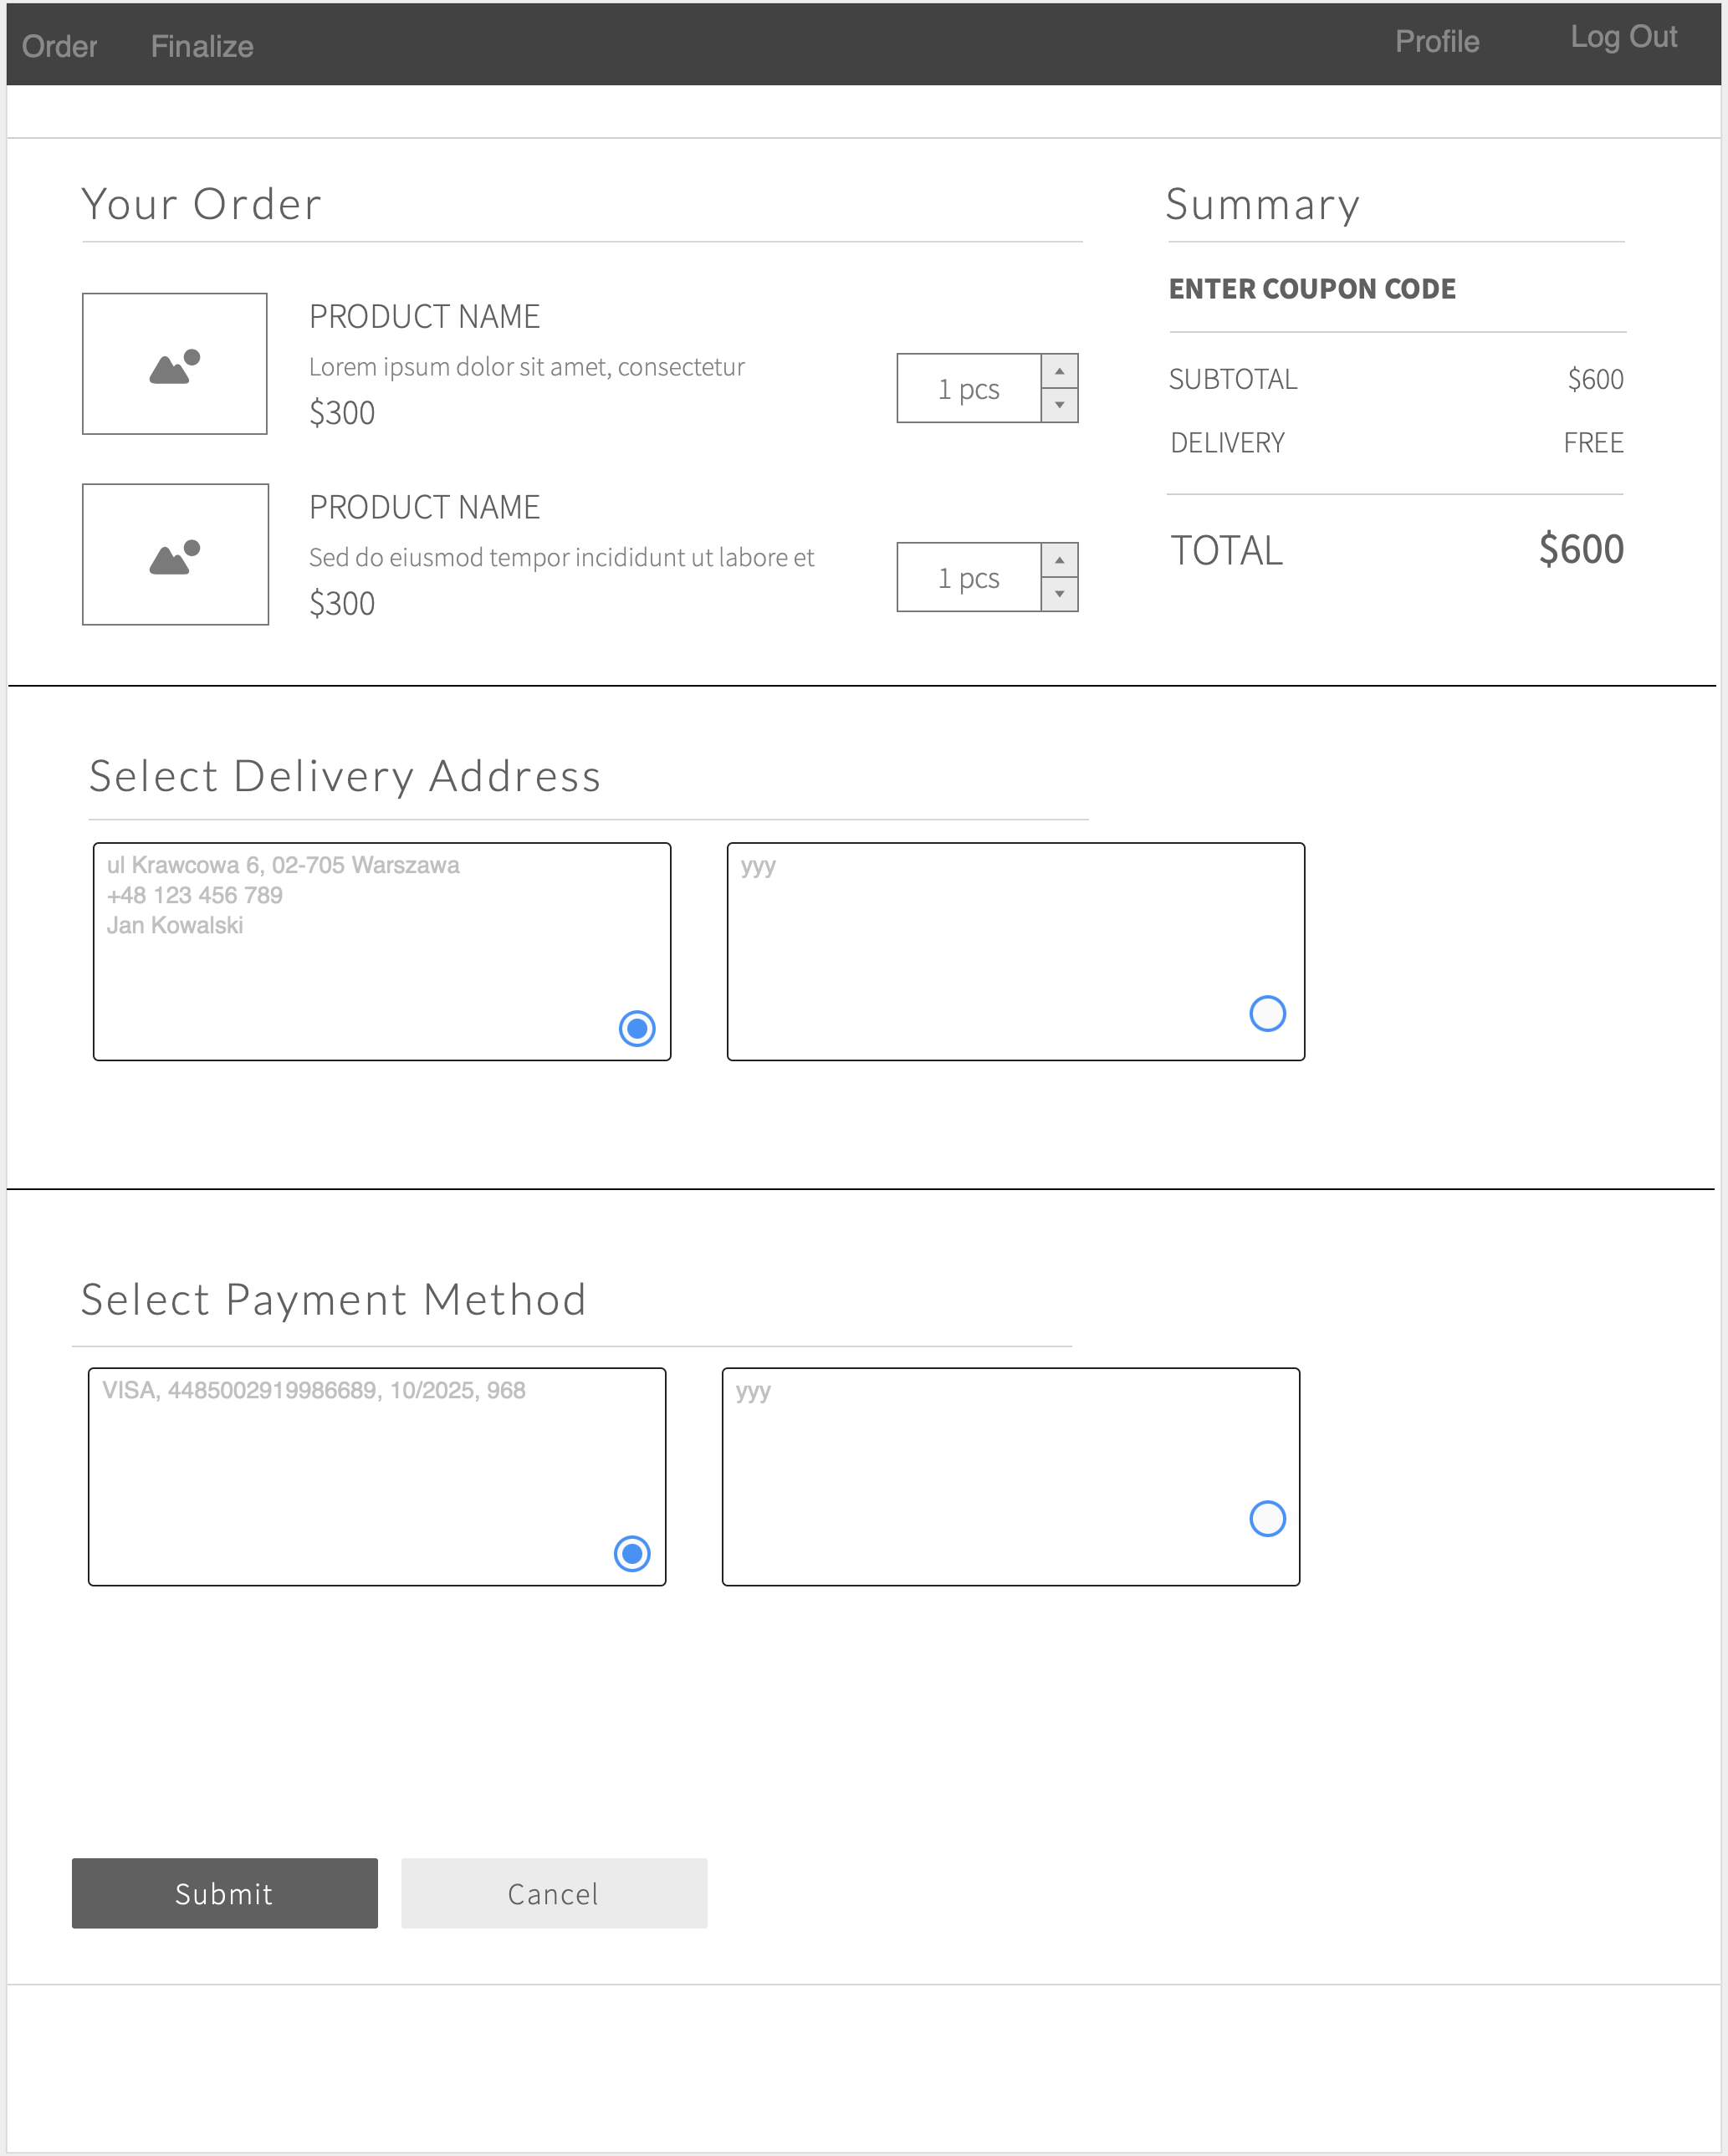
\includegraphics[width=0.7\linewidth]{mockups_fragment.png}
    \caption{Fragment makiety interfejsu użytkownika}
    \label{fig:mockups}
\end{figure}
